%%%%%%%%%%%%%%%%%%%%%%%%%%%%%%%%%%%%%%%%%%%%%%%%%%%%%
\documentclass[apj]{emulateapj}
%\documentclass[preprint2]{aastex61}
%\documentclass[12pt,preprint]{aastex}
\graphicspath{{figures/}}
\DeclareGraphicsExtensions{.jpg,.pdf,.png,.eps,.ps}

\usepackage[table,usenames,dvipsnames]{xcolor}
%\usepackage{amsmath}
%\usepackage{subfigure}
\usepackage[backref,breaklinks,colorlinks,citecolor=blue]{hyperref}
\usepackage{natbib}
%\usepackage{natbib}
\bibliographystyle{fapj}
%\usepackage{graphicx}
%\usepackage{multirow}
\usepackage{soul}

%\newcommand{\jcap}{JCAP}

\newcommand{\sqdeg}{deg$^2$ }
\newcommand{\omb}{\ensuremath{\Omega_b h^2}}
\newcommand{\omc}{\ensuremath{\Omega_c h^2}}
\newcommand{\clpp}{\ensuremath{C_{L}^{\phi\phi}}}
\newcommand{\cpmf}{\ensuremath{C_{\ell}^{\rm PMF}}}

\newcommand{\cpmftens}{\ensuremath{C_{\ell}^{\rm PMF,\,tens}}}
\newcommand{\cpmfvec}{\ensuremath{C_{\ell}^{\rm PMF,\,vec}}}
\newcommand{\apmf}{\ensuremath{A_{\rm PMF}}}
\newcommand{\bpmf}{\ensuremath{B_{\rm 1\,Mpc}}}
\newcommand{\alens}{\ensuremath{A_{\rm lens}}}
\newcommand{\lcdm}{\ensuremath{\Lambda}CDM}
\newcommand{\nrun}{\ensuremath{n_{\rm run}}}
\newcommand{\neff}{\ensuremath{N_{\rm eff}}}
\newcommand{\ho}{H\ensuremath{_0}}
\newcommand{\mnu}{\ensuremath{\sum m_\nu}}
\newcommand{\ukarcmin}{\ensuremath{\mu}{\rm K-arcmin}}
\newcommand{\lknee}{\ensuremath{\ell_{\rm knee}}}
\newcommand{\fermilat}{\textit{Fermi}-LAT}

\newcommand{\be}{\begin{equation}}
\newcommand{\ee}{\end{equation}}
\newcommand{\planck}{{\sl Planck}}
\newcommand{\wmap}{{\sl WMAP}}
\newcommand{\bicepkeck}{BICEP2/Keck Array}
\newcommand{\sptnew}{SPT-3G}
\newcommand{\pb}{\textsc{Polarbear}}
\newcommand{\simons}{Simons Array}
\newcommand{\sptpol}{SPTpol}
\newcommand{\advactpol}{Adv.~ACTpol}

\newcommand{\tbd}[1]{\textcolor{Red}{{\bf TBD}: #1}}
\newcommand{\gab}[1]{\textcolor{Orchid}{[{\bf GS}: #1]}}
\newcommand{\changed}[1]{\textcolor{Red}{#1}}
\newcommand{\removed}[1]{\textcolor{Red}{}}
\include{number_list}

%

% ref to section \S\ref{sec:label}

%\submitjournal{ApJ}
\def\Melbourne{1}
\def\uci{2}
%%%%%%%%%%%%%%%%%%%%%%%%%%%%%%%%%%%%%%%%%%%%%%%%%%%%%
\begin{document}

\title{Cosmic Microwave Background Power Spectra from Few Bit Timestreams}
\author{L.~Balkenhol\altaffilmark{\Melbourne} and C.~L.~Reichardt\altaffilmark{\Melbourne}}
\altaffiltext{\Melbourne}{School of Physics, University of Melbourne, Parkville, VIC 3010, Australia}
\email{christian.reichardt@unimelb.edu.au}

\begin{abstract} % copied off ASA for now
Observations of the Cosmic Microwave Background (CMB) are of immense value to modern cosmology. However, future CMB experiments must confront challenges in mission planning, hardware and analysis that arise from the sheer size of the time-ordered-data being recorded. These challenges are particularly significant for Antarctic and satellite experiments which depend on satellite links to transmit the data. We investigate using extreme digitisation to address these challenges. Unlike lossless compression, extreme digitisation introduces additional noise into the data. We present an optimal 1, 2 and 3 bit digitisation schemes and lay out how the added noise varies between the schemes and as a function of hits per pixel in the map for temperature and polarisation observations. We show that the noise penalty of 3 bit digitisation is at the percent-level for CMB power spectrum measurements. This is impressive considering that it would reduce the data volume by an order of magnitude. We argue that extreme digitisation is a promising strategy for upcoming experiments.
\end{abstract}

\keywords{ cosmic background radiation --- polarization }
\section{Introduction}
\label{sec:intro}

Observations of the Cosmic Microwave Background (CMB) have played a key role since 1964 (discovery paper). Current and future CMB experiments will continue to deliver new insights by studying the temperature and polarisation information contained in the CMB. These will constrain help putting tighter constraints on cosmological models. The most prominent science goal is the discovery of the imprint left by inflationary gravitational waves. Additionally studies of CMB lensing and the Sunyaev-Zeldovich (SZ) effects will deliver new insight. CMB experiments however also provide a valuable counterpart to ground-based particle physics experiments, as they probe the relativisitc number of species, the helium fraction and the neutrino mass sum.

The outstanding contribution of CMB science to modern physics has demanded a high standard of data analysis. The CMB community has developed a variety of compression and computational techniques to manage the increasing influx of data, while maximising the science output. These include the compression of time-ordered data into maps, bandpower estimation and the pseudo Cl method.

A growing hurdle for experiments at remote locations are the transmission limitations of satellite links. Space-based experiments have employed a combination of lossless and lossy compression techniques, including reduced bits in the time-ordered-data (TOD). Antarctica based experiments that transmit a portion of their data via a satellite link have downsampled their TOD in the past to meet their telemetry requirements. They have yet to exploit few bit digitisation of the TOD.

As we approach the next generation of ground-based experiments, Stage-4, and the launch of a new generation of space-based missions (liteBIRD, PIXIE, COrE+), we must treat the transmission bottleneck carefully. Without a review of the current compression techniques employed we are sure to lose information.

In this work we present the method of extreme digitisation, which compresses a rich digital input signal and compresses it into a few bits. We apply extreme digitisation to the TOD and detail its effect on temperature and polarisation observations. We find that an optimal 3-bit digitisation scheme adds as little as $\sim 2\%$ to the map noise level. While the digtisation schemes described here are primarily laid out for ground-based Stage-4 experiments, future space-based missions must inevitably study lossy compression techniques.

This work is structured as follows. We detail the arising challenges in handling large TOD in \S\ref{subsec:problem}. We subsequently formulate extreme digitisation formerly in \S\ref{subsec:extremedigitisation} and lay out the framework used to test the performance of this compression technique in \S\ref{subsec:method}. In \S\ref{sec:results} we present the results obtained. We summarize our findings in \S\ref{sec:conclusions}. 



%CMB is great; One reason is that there is a history of compression and computational techniques that reduce the load of large datasets. ie maps; bandpowers; pseudo-cls.

%satellites have also reduced bits on TOD; ground based haven't had to yet

%however as we discuss building ever larger arrays at remote sites, we are starting to be limited: spt example.

%in this work we present digitisation for ground-based cmb polarisation measurements.
%teaser results


%The outline of this paper is as follows. 
%We present the digisation schemes in \S\ref{sec:dig}, and their performance in \S\ref{sec:results}
%We summarize our findings in \S\ref{sec:conclusions}. 

\section{Digitisation}
\label{sec:dig}

\subsection{Problem}
\label{subsec:problem}

%Data influx + Transmission

The science goals of upcoming CMB experiments naturally lead to a large influx of data. To achieve them longer observations with more detectors are needed. However, the best observations sites for CMB observations are at remote locations: in space and in the Antarctica. Experimetns at these locations depend on satellite transmission The next generation of ground-based experiments, Stage-4, will aim to collect 2 million detector years worth of data. A Stage-4 style experiment will face a data influx of $\sim O(10)Tb/d$. However, the current transmission allocation for the SPT3G is at $150Gb/d$. SPT3G currently deals with its transmission bottleneck by downsampling the TOD, i.e. discarding high frequency information. While this will likely see an increase going into the next stage of experimetns it will not be able to over the entire observation. Going into Stage-4 we anticipate that compression rates for transmission must increase by an order of magnitude. Continued use of heavy downsampling will narrow the informatino window decisively - prohibiting high l science to be carried out on the transmitted dataset. This also means that any potential faults or errors in the experiment that only become visible in high frequencies will go unnoticed for longer.

Similarly, future space-based missions (PIXIE, COrE+, liteBIRD) aim to increase their detector count by at least an order of magnitude compared to PLANCK. It is questionable whether their telemetry specifications will allow for transmission of the data with PLANCK-style compression. Methods of storing large amounts of data on upcoming satellites will likely be prohibited by financial decisions: the amount of storage space required becomes financially relevant at the scales targeted.

%Planning

Beyond these transmission hurdles detailed mission planning is becoming exceedingly expensive. As noted by (S4 science book) a full simulation of TOD over the entire parameter space of detection scenarios for numerous set-ups is the desired way to plan Stage-4 configuration. Similarly space-based missions must carry out a similar analysis to optimise their science out-put. However, given the sheer size of TOD this is not possible. We must turn to different planning strategies or aim to reduce the size of the TOD in order to maximise the productivity of planning and development stages.

Operations on the TOD, such as noise-removal or map-making are a vital part of CMB data analysis. Through the expontentially growing size of TOD CMB data analysis is becoming increasingly expensive.

%why is it worth considering

Extreme Digitisation would tackle the challenges mentioned above by recuding the size of the TOD by an order of magnitude. Together with already exploited lossless compression techniques (such as FLAC) this will directly tackle transmission hurdles. While it needs to be investigated to what extent existing algorithms can be carried over, extreme digitisation has the possiblity of solving planning and analysis problems.

\subsection{Extreme Digitisation}
\label{subsec:extremedigitisation}

% rephrase these, basically off Max1978

Digitisation is a lossy compression technique. However the induced noise depends on the number of bits used, the digitisation thresholds and the output levels chosen. To minimise the noise induced through this process one must know the nature of input signal. A theoretical framework to obtain these levels was laid out by Max in 1978. We review the key aspects of his work relevant to our findings below.

We divide the space $-\infty \to \infty$ into $N$ ranges. One then has endpoints $x_k$ and output levels $y_k$, such that an input between $x_i$ and $x_{i+1}$ produces an output at $y_i$. Conventionally one chooses $x_{1} = -\infty$ and $x_{N+1} = \infty$. In order to determine an optimal set of $x_k$ and $y_k$ we would like to minimise the distortion

\[ D = \left\langle  \left( s_{in} - s_{out} \right)^2 \right\rangle \]

For a given input amplitude probability density $p(x)$ we may rewrite the above as

\[ D = \sum_{i = 1}^N \int_{x_i}^{x_{i+1}} \left(x-y_i\right)^2 p(x) dx \]

Seeing as we wish to minimise the distortion we differentiate the above with respect to $x_i$ and $y_i$ and set the derivatives to zero.

\[ \frac{\partial D}{\partial x_i} = \left(x_i-y_{i-1}\right)^2 p(x_i) - \left(x_i - y_i\right)^2 p(x_i) = 0 \]

\[ \frac{\partial D}{\partial x_j} = -2 \int_{x_i}^{x_{i+1}} \left( x-y_i \right) p(x) dx = 0 \]

From the first equation above we deduce that

\begin{equation} \label{eq:digitequalspacecondition}
x_i = \frac{y_i+y_{i+1}}{2}
\end{equation}

The second one

\begin{equation} \label{eq:digitareacondition}
\int_{x_i}^{x_{i+1}} \left( x-y_i \right) p(x) dx = 0
\end{equation}

implies that we should choose $y_i$, such that it halves the area underneath $p(x)$ in the interval $x_i \to x_{i+1}$.

We are interested in the case where our input signal can fairly be approximated by gaussian white noise, i.e. $p(x) = 1/sqrt{2\pi} e^{-x^2/2}$. Even with these assumptions we cannot solve the resulting equations analytically. Instead one can begin by picking $y_1$ and calculating the remaining $x_i$ and $y_i$ using equation \ref{eq:digitequalspacecondition}. One then observes weather this choice of values satisfy the conditions given by equation \ref{eq:digitareacondition}. If that is the case the $x_k$ and $y_k$ were chosen appropriately. This is unlikely to succeed on the first try. We rather solve the above system iteratively.

This was carried out by Max. We incorporate his results by formulating the multi-level functions we use for our 1, 2 and 3 bit digitisation process. For 1 bit digitisation we apply the sign function

\[ \hat{x}(t) = \left\{ \begin{array}{lr}
1, & \text{for } x(t) > 0\\
-1, & \text{for } x(t) \leq 0
\end{array} \right. \]

to the TOD. For 2 bit digitisation we apply the four-level function

\[ \hat{x}(t) = \left\{ \begin{array}{lr}
1.51 \sigma, & \text{for } x(t) \geq 0.9816 \sigma\\
0.4528 \sigma, & \text{for } 0 \leq x(t) < 0.9816 \sigma\\
-0.4528 \sigma, & \text{for } 0.9816 \sigma \leq x(t) < 0\\
-1.51 \sigma, & \text{for } 0.9816 \sigma < x(t)\\
\end{array} \right. \]

Finally the optimal 3 bit digitisation is described by the eight-level function

\[ \hat{x}(t) = \left\{ \begin{array}{lr}
2.152 \sigma, & \text{for } x(t) \geq 1.748 \sigma\\
1.344 \sigma, & \text{for } 1.05 \sigma \leq x(t) < 1.748 \sigma\\
0.756 \sigma, & \text{for } 0.501 \sigma \leq x(t) < 1.05 \sigma\\
0.245 \sigma, & \text{for } 0 \leq x(t) < 0.501 \sigma\\
-0.245 \sigma, & \text{for } 0.501 \sigma \leq x(t) < 0\\
-0.756 \sigma, & \text{for } 1.05 \sigma \leq x(t) < 0.501 \sigma\\
-1.344 \sigma, & \text{for } 1.748 \sigma \leq x(t) < 1.05 \sigma\\
-2.152 \sigma, & \text{for } 1.748 \sigma < x(t)\\
\end{array} \right. \]

% Theoretical lvls for gaussian white noise

\subsection{Methods}
\label{subsec:method}

To investigate the performance of the aforementioned digitisation schemes we simulate many scans over CMB template maps at the timestream level. Each scan is performed by a single detector. We obtain maps that use 64bit TOD and maps that have undergone 1, 2 and 3 bit digitisation at the timestream level. We calculate the temperature and polarisation power spectra of each map and determine the additional noise induced through the extreme digitisation process.

The $I, Q, U$ template maps used were created through healpy's synfast. As the input power spectra we use the results by Placnk 2015. The underlying cosmological parameters are summarised in table \ref{tab:inputcosparams}.

We simulate observing a $\sim 600$ \sqdeg patch of the sky. To do so we perform constant elevation scans (CES) over the observation region. We repeat the observation strategy $100$ times with a slight offset in RA and DEC each time, such that all pixels within the path are hit approximately uniformly. 

While performing each CES the appropriate pixels that are being targeted are determined. The corresponding values from the template maps are then accessed and added to realisations of the detector noise of appropriate length. We assume the detector noise to be gaussian white noise.

The constructed timestreams for $I$, $Q$ and $U$ are then compressed in 4 different ways: averaging of the timestream, representing each datapoint as a 64bit floating point number and applying the three introduced digitisation schemes before averaging the timestream. The simulation parameters are summarised in table \ref{tab:modelparams}. Through this procedure we slowly build up 12 different maps: three maps that corresponds to a normal scan over the polarised CMB and 9 maps that reconstruct the observed patch from an extremely compressed time-ordered data. Additionally we retain the hitmap.

The simulation described above was implemented in Python 2.7. It has considerable computational requirements if we want to reach up to $\sim 10^8$ hits per pixel. To carry out this simulation we make use of parallelisation and the computing power provided by NERSC.

\begin{table}[tbh]
\begin{center}
\caption{\label{tab:inputcosparams} Input Cosmological Parameters}
\small
\begin{tabular}{l | c c c }
$\Omega$ & XX&XX&$r$\\
\hline

\end{tabular}
\tablecomments{ 
Cosmological parameters used to create the template maps.
} \normalsize
\end{center}
\end{table}

\begin{table}[tbh]
\begin{center}
\caption{\label{tab:modelparams} Assumed Survey Parameters}
\small
\begin{tabular}{c c c c c}
$\mathrm{NSIDE}$ & $f_{readout}$ & $f_{sky}$ & $\sigma^{\mathrm{T}}_{detector}$ & $\sigma^{\mathrm{Pol}}_{detector}$\\
\hline
$4096$ & $200\mathrm{Hz}$ & $\sim 0.014$ & $500\mathrm{K}\sqrt{\mathrm{s}}$ & $\sqrt{2}\times500\mathrm{K}\sqrt{\mathrm{s}}$\\

\end{tabular}
\tablecomments{ 
Parameters used in the simulated sky strategy. The RA speed is tweaked to match the desired hits per pixel.
} \normalsize
\end{center}
\end{table}



\section{Results}
\label{sec:results}

\subsection{Analysis}
\label{subsec:analysis}

We use PolSpice to compute the $TT, EE, BB$ power spectra of the obtained maps. When doing so we apodise the observed skypatch using a cosine mask to minimise cut sky effects on the spectra. Please see \ref{tab:polspiceparams} for an overview of the parameters used in this process.

\begin{table}[tbh]
\begin{center}
\caption{\label{tab:polspiceparams} PolSpice Parameters}
\small
\begin{tabular}{c c c c}
weightfile & apodizesigma & apodizetype & polarization \\
\hline
cosine mask & $\sqrt{600}/2$ & 1 & YES \\

\end{tabular}
\tablecomments{ 
Parameters used when calling PolSpice to calculate the power spectra. Remaining parameters have been left at their default value.
} \normalsize
\end{center}
\end{table}

The obtained power spectra originating from digitised time streams are normalised against the power spectra that use the full time stream data. We use results that originate from $\sim 10^8hpp$ maps. We separately normalise the TT, EE and BB spectra. The normalisation constant obtained from this calculation are then applied to all lower hit per pixel runs.

We restrict ourselves to windows in multipole space where we trust that the spectra are within appropriate multipole moment range given the patch size and are signal dominated. We therefore place a lower limit on the normalisation window for each channel from

\[ l = \frac{2}{\pi} \frac{(180^\circ )^2}{600 sqdeg} \approx 35 \]

where we have rounded up to the next highest integer. We find the upper bound on the normalisation window by demanding that

\[ \frac{C_l^{S}}{C_l^{N}} \geq 10 \]

\subsection{Additional Noise}
\label{subsec:additionalnoise}

To determine how much the quality of the power spectra suffers due to the digitisation we would like to compare the map noise levels. We would like to put this value into context with the map noise level induced through the detector noise. We therefore formulate

\[ \frac{\Delta \sigma}{\sigma} = \frac{\sigma_{MAP}^{D}-\sigma_{MAP}^{SN}}{\sigma_{MAP}^{SN}} \]

where $\sigma_{MAP}^{SN}$ is the map noise level of the full power spectra (signal plus noise) and $\sigma_{MAP}^{D}$ is the map noise level obtained from the power spectra originating from extremely digitised TOD. We assume that the digitisation process results in adding some constant  to the powerspectrum, i.e.

\[ C_l^D = C_l^N + C_l^X \]

in the limit where we are dominated by noise. Here $C_l^D$ is the power spectrum originating from a digitised timestream, $C_l^N$ is the detector noise level and $C_l^X$ the additional noise induced. We may now progress with

\[\frac{\Delta \sigma}{\sigma} = \sqrt{\frac{C_l^D}{C_l^{N}}} - 1  = \sqrt{\frac{C_l^N + C_l^X}{C_l^{N}}} - 1 = \sqrt{1 + \frac{C_l^X}{C_l^{N}}} - 1  \]

Before analysing $C_l^X/C_l^N$ we rebin the power spectra to $\Delta l = 123$. This guarantees that the points in the noise tail are independent of one another, allowing us to extract an uncertainty for the above quantity.

The results for the 1, 2 and 3 bit digitisation schmes for the TT, EE and BB power spectra are summarised in \ref{fig:extranoise}. We would like to points out three key results. Firstly, 3 Bit digitisation performs the best, followed by 2 Bit and finally 1 Bit digitisation. This is what we expect, given that with each additional bit we may retain more information. Secondly, for a fixed detector noise level, the additional percentage to the map noise level due to digitisation is independent of the number of hits per pixel. This is a valuable result, as it means that there is not a certain point at which surveys start becoming viable for this compression techniques, but they rather perform equally well throughout the range of hits per pixel tested. Lastly, the added noise levels are astonishingly low.

%Any other results that are outstanding

%? Analysis result: To uncertainty in cosmological parameters?

We present the average additional percentage to the map noise level through digitisation in \ref{tab:noise}. These results are obtained by calculating the weighted average across all hits per pixel for a given digitisation scheme and channel. We note that an optimal 3 bit digitisation scheme adds as little as $\sim2\%$ to the map noise level.

Given that advances in CMB observations happen in order magnitude jumps between generations of experiments this is a negligible noise addition, considering that it reduces the TOD by an order of magnitude.

Extreme digitisation is a viable lossy compression technique when dealing with large low signal to noise, slowly varying datasets. Within this limit digitisation relies on the noise to push the small signal towards the correct side of the locally stationary signal. A low signal to noise ratio prevents us from a signal saturating the digitisation levels. For large datasets are needed to provide many samplings of each locally stationary signal. An increase in bit number does not necessarily improve the recovery of the mean, but rather advances narrowing down on its uncertainty, by improving the nulling out of the noise. Improving the number of samples in a dataset improves the finding of the mean, as it allows for more correctly pushed digitised points to be considered.

\begin{figure*}[htb]\centering
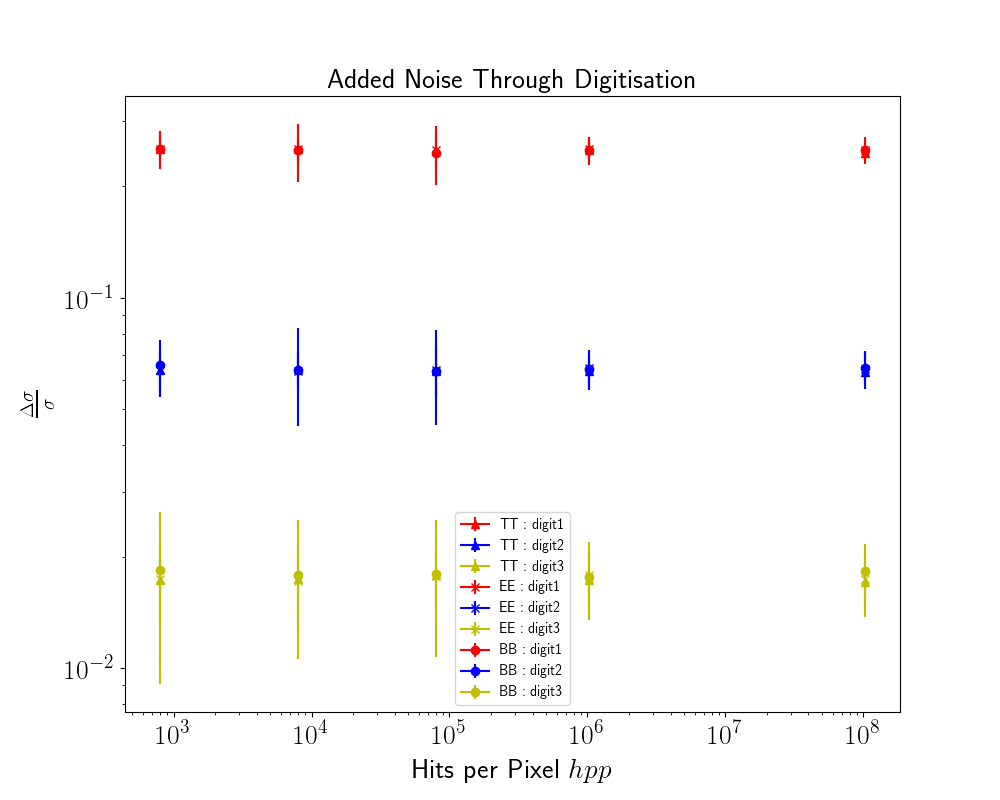
\includegraphics[width=0.9\textwidth,clip]{Plots/addednoise.png}
  \caption[Current ]{
  Addition to the map noise level due to digitisation. 
           \label{fig:extranoise}
  }
\end{figure*}

\begin{table}[tbh]
\begin{center}
\caption{\label{tab:noise} Noise levels}
\small
\begin{tabular}{l | c c c }
 Channel & 1 Bit & 2 Bit & 3 Bit\\
 \hline
 TT & & & \\
 EE & & & \\
 BB & & & \\

\end{tabular}
\tablecomments{ 
Added percentage to the map noise level due to digitisation.
} \normalsize
\end{center}
\end{table}

\begin{table*}[tbh]
\begin{center}
\caption{\label{tab:experiments} Assumed survey parameters}
\small
\begin{tabular}{l || c c c c c }
Experiment & Sky coverage & Polarized Noise level  & 1/$f$ knee & Beam FWHM \\
& &($\mu$K-arcmin)&&(arcmin.)\\
\hline
\tiny \\ \small
CMB Stage III & & & & \\
~~~~~SPT-3G & 6\% & 3.0 & 200 & 1.2 \\
~~~~~Simons Array & 36\% & 9.5 & 200 & 3.5 \\ 
\tiny \\ \small
%\hline
CMB Stage IV & 55\% & 1.3 & 100 & 4.0 \\
\end{tabular}
\tablecomments{ 
Key numbers about the planned stage III and IV experiments. 
The sky coverage percentages are after galactic cuts. 
Unless otherwise noted,  the Fisher matrix forecasts in this work use these numbers. 
All forecasts also allow for beam and calibration uncertainties as noted in the text. 
} \normalsize
\end{center}
\end{table*}

\section{Conclusions}
\label{sec:conclusions}

In this work we have demonstrated the power of digitising CMB TOD from 64-bit down to few-bits. The additional noise induced through this step was at the percent-level for chosen optimal digitisation schemes for temperature and polarisation observations.

The motivation behind employing extreme digitisation is the reduction of TOD by an order of magnitude. This primarily addresses challenges in data transmission that will face upcoming CMB experiments at remote locations. Benefits in planning and analysis seem feasible.

Future work on investigating this compression technique must aim to understand the nature of the induced noise better. For this the performance of cluster-finding algorithms is interesting.

It should be laid out how this changes when moving to a more realistic noise profile. We do not expect this to alter the practicality of our results - even if a moderate change in the noise profile doubles the additional percentage to the map noise level extreme digitisation is still practical. Ideas on how to deal with 1/f noise, e.g. chunking of the data before applying extreme digitisation have already been investigated by Planck. These thoughts should be considered when designing the compression schemes of future space-based CMB missions, which will be unable to recover their full data with latency, but rather fully rely on the transmitted data.

\acknowledgments % thank patrick for discussion/starting point? Andrew?

We thank the \changed{referee as well as} Srinivasan Raghunathan and Federico Bianchini for valuable feedback on the manuscript. 
We acknowledge support from an Australian Research Council Future Fellowship (FT150100074), and also from the University of Melbourne. 
This research used resources of the National Energy Research Scientific Computing Center, which is supported by the Office of Science of the U.S. Department of Energy under Contract No. DE-AC02-05CH11231. 
We acknowledge the use of the Legacy Archive for Microwave Background Data Analysis (LAMBDA). Support for LAMBDA is provided by the NASA Office of Space Science.


\bibliography{digitisation}


\end{document}
